%%%%%%%%%%%%%%%%%%%%%%%%%%%%%%%%%%%%%%%%%%%%%%%%%%%%%%%%%%%%%%%%%%%%%%%%%%%%%%%%%%%%%%%%%%%%%%%
%                                        SEGMENTATION                                         %
%%%%%%%%%%%%%%%%%%%%%%%%%%%%%%%%%%%%%%%%%%%%%%%%%%%%%%%%%%%%%%%%%%%%%%%%%%%%%%%%%%%%%%%%%%%%%%%
\chapter{Deformable Shape Models using Deep Learning}
\label{chap:seg}

\begin{chapabstract}
 Coucou
\end{chapabstract}

\vspace{1cm}

{   
    \setstretch{1.0}
    \minitoc
}

\newpage

%%%%%%%%%%%%%%%%%%%%%%%%%%%%%%%%%%%%%%%%%%%%%%%%%%%%%%%%%%%%%%%%%%%%%%%%%%%%%%%%%%%%%%%%%%%%%%%
\section{Deformable shape models}

\subsection{Before deep learning}

\begin{itemize}
    \item Link with registration ?
\end{itemize}

\subsection{Building a shape model}

\subsection{Deforming the shape model}

An Unsupervised Learning Model for Deformable Medical Image Registration



%%%%%%%%%%%%%%%%%%%%%%%%%%%%%%%%%%%%%%%%%%%%%%%%%%%%%%%%%%%%%%%%%%%%%%%%%%%%%%%%%%%%%%%%%%%%%%%
\section{Deformable shape models and deep learning}

We propose in this section to train a neural network to predict the deformation required for a shape model to match a specific segmentation target on a specific image. There are three components: learning a global transformation 

\begin{figure}[htbp]
	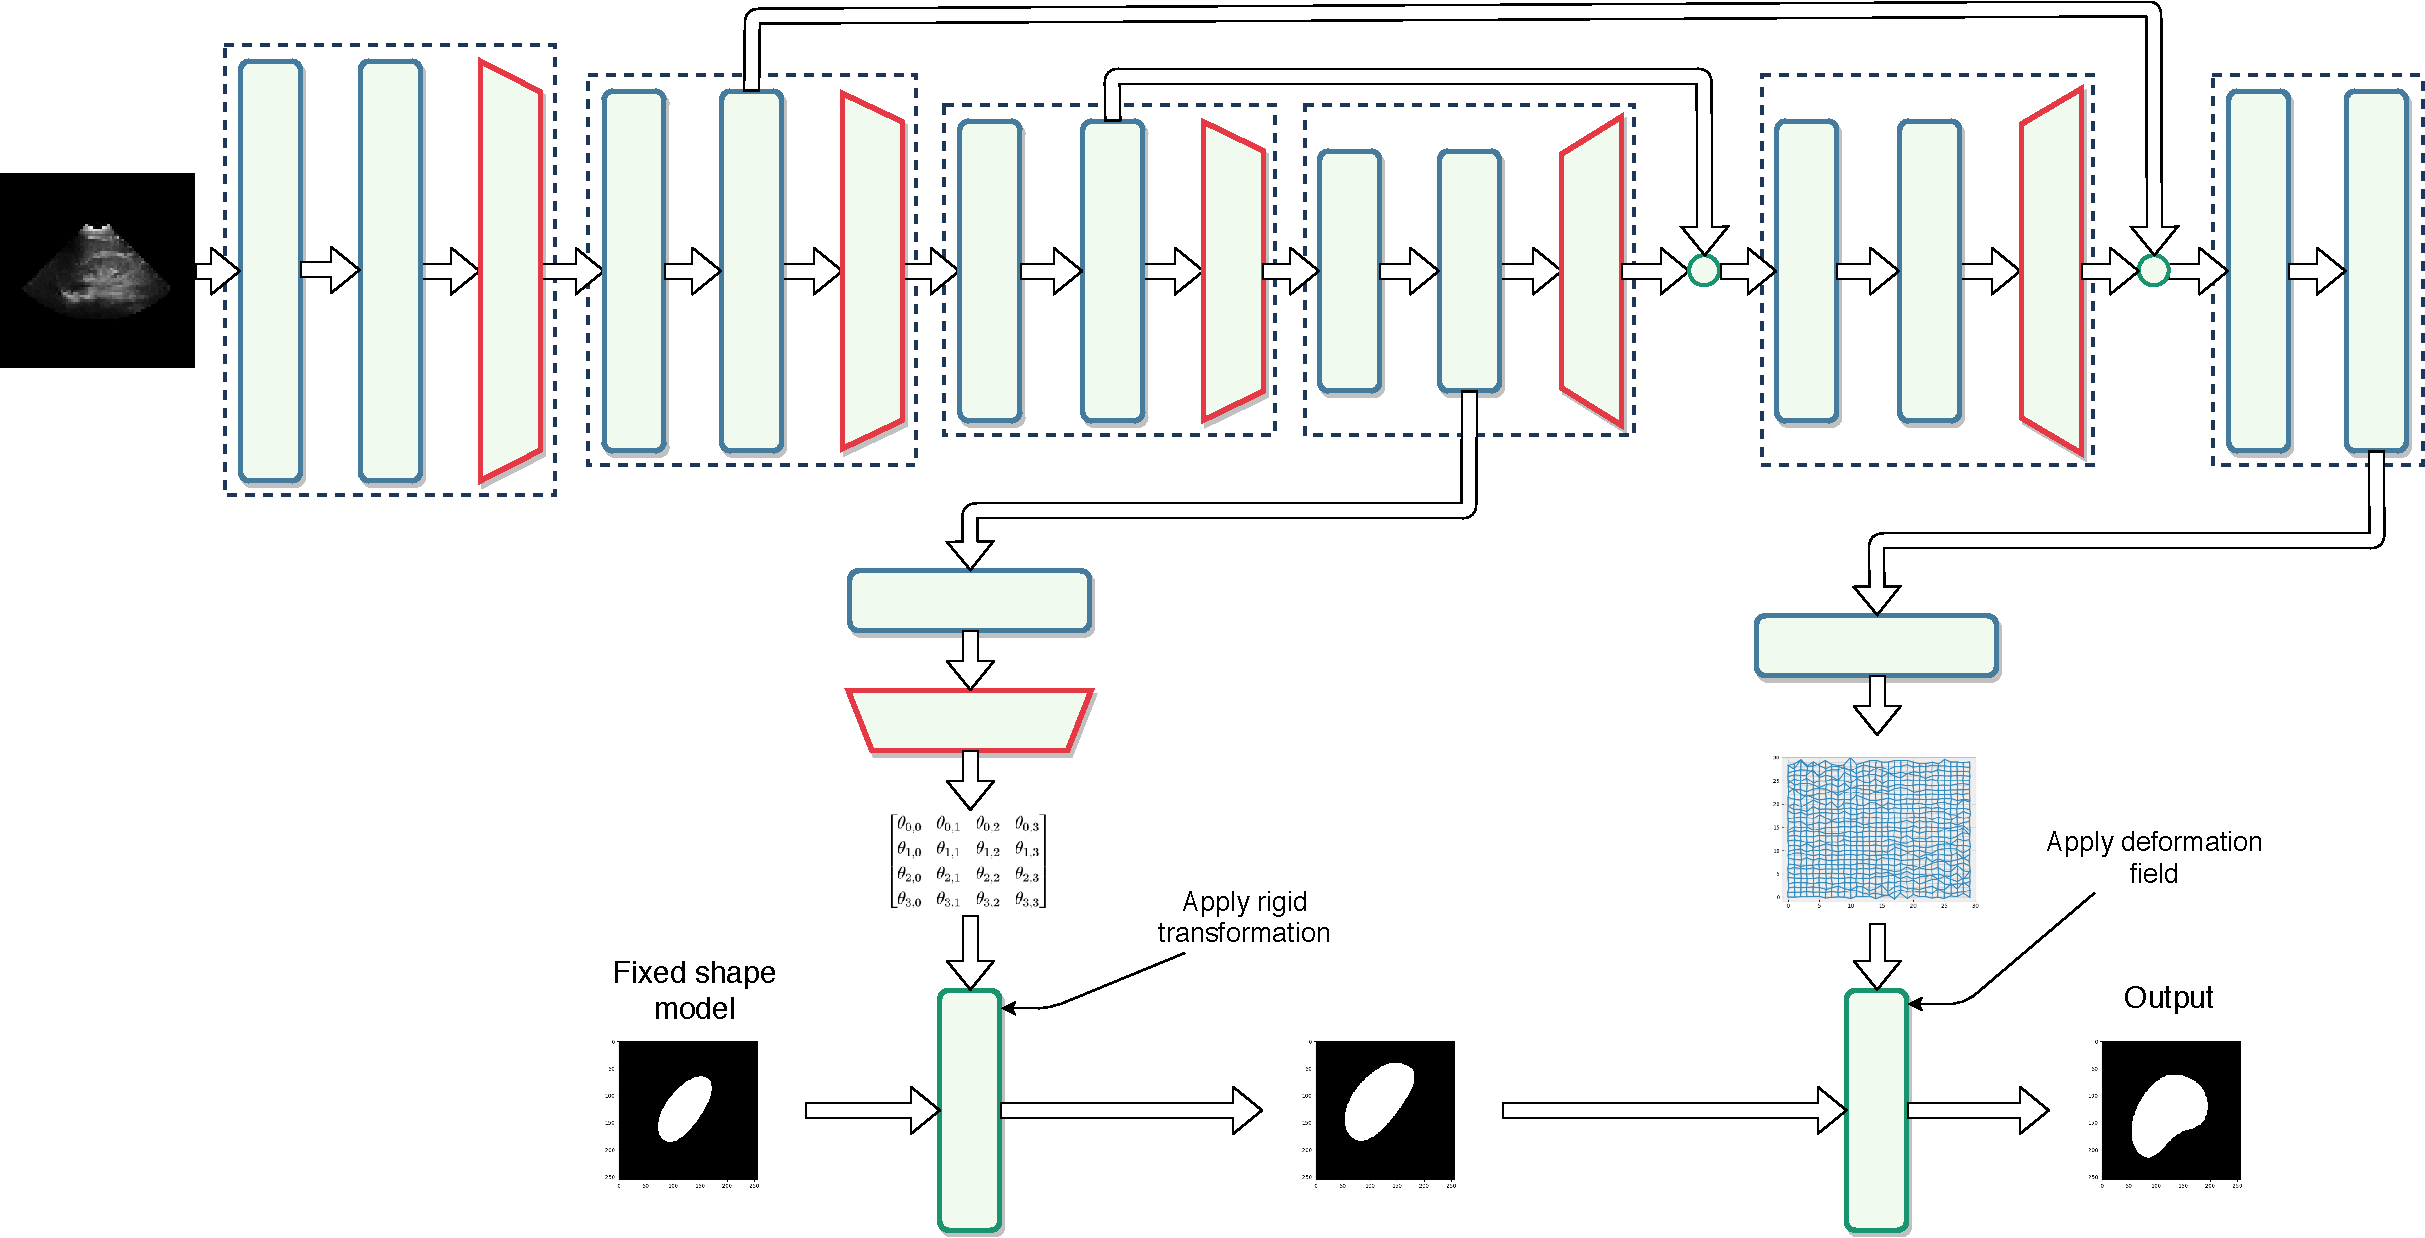
\includegraphics[width=\textwidth]{img_seg/deformation_network}
    \caption{Intensity Layer. ``Parameters Prediction'' can be any model, in our case it is a 3-layers ConvNet.}
    \label{fig:deform_network}
\end{figure}

\subsection{Learning a global transformation}

\begin{equation}
    \begin{bmatrix}
    \theta_{0, 0} & \theta_{0, 1} & \theta_{0, 2} & \theta_{0, 3} \\
    \theta_{1, 0} & \theta_{1, 1} & \theta_{1, 2} & \theta_{1, 3} \\
    \theta_{2, 0} & \theta_{2, 1} & \theta_{2, 2} & \theta_{2, 3} \\ 
    \theta_{3, 0} & \theta_{3, 1} & \theta_{3, 2} & \theta_{3, 3} 
    \end{bmatrix}
\end{equation}

- using a global transformation

\subsection{Learning a deformation field}

- predicting the deformation field

\subsection{Distance map and loss}

- Distance map and appropriate loss

%%%%%%%%%%%%%%%%%%%%%%%%%%%%%%%%%%%%%%%%%%%%%%%%%%%%%%%%%%%%%%%%%%%%%%%%%%%%%%%%%%%%%%%%%%%%%%%
\section{Application to the segmentation of the kidney in 3D-US}

- dataset and preprocessing

TODO:
\begin{itemize}
    \item Compare global transfo alone, defo field alone, global + field
\end{itemize}


